\documentclass[xcolor=dvipsnames]{beamer}

\usetheme{AnnArbor}
\usepackage{dsfont}
\usepackage{amsmath}
\usepackage{caption}
\usepackage{hyperref}
\usepackage{xcolor}
\usepackage{color}
\usepackage{commath}
\usepackage{physics}
\usepackage{enumerate}
\usepackage{hyperref}
\usepackage{graphics}
\usepackage{graphicx}
\usepackage{subcaption}
\usepackage{lmodern}
%\usepackage[T1]{fontenc}

\newcommand{\customcite}[1]{\citeauthor{#1} (\citeyear{#1})}
\newtheorem{satz}{Satz}

\usecolortheme{seagull}
\setbeamertemplate{footline}[page number]
\setbeamercolor{frametitle}{fg=blue,bg=White}

%\usepackage[backend=bibtex, style=authoryear-comp]{biblatex}

\setbeamertemplate{bibliography item}{\insertbiblabel}
\beamertemplatenavigationsymbolsempty
%\bibliographystyle{IEEEtran}

\usepackage[style=authoryear]{biblatex}
\renewcommand*{\nameyeardelim}{\addcomma\addspace}
\addbibresource{\jobname.bib}

\usepackage{filecontents}
\begin{filecontents}{\jobname.bib}
@incollection{aldous1985exchangeability,
  title={Exchangeability and related topics},
  author={Aldous, David J},
  booktitle={{\'E}cole d'{\'E}t{\'e} de Probabilit{\'e}s de Saint-Flour XIII—1983},
  pages={1--198},
  year={1985},
  publisher={Springer}
}
@Article{quanteda,
  title = {quanteda: An R package for the quantitative analysis of textual data},
  journal = {Journal of Open Source Software},
  author = {Kenneth Benoit and Kohei Watanabe and Haiyan Wang and Paul Nulty and Adam Obeng and Stefan Müller and Akitaka Matsuo},
  doi = {10.21105/joss.00774},
  url = {https://quanteda.io},
  volume = {3},
  number = {30},
  pages = {774},
  year = {2018},
}
@article{blei2012probabilistic,
  title={Probabilistic topic models},
  author={Blei, David M},
  journal={Communications of the ACM},
  volume={55},
  number={4},
  pages={77--84},
  year={2012},
  publisher={ACM New York, NY, USA}
}
@online{blei2012presentation,
  title={Probabilistic topic models},
  author={Blei, David M},
  url={http://www.cs.columbia.edu/~blei/talks/Blei_ICML_2012.pdf},
  date={2012-06-26},
  urldate={2020-07-14}
}
@article{blei2003latent,
  title={Latent dirichlet allocation},
  author={Blei, David M and Ng, Andrew Y and Jordan, Michael I},
  journal={Journal of machine Learning research},
  volume={3},
  number={Jan},
  pages={993--1022},
  year={2003}
}
@article{lucas2015computer,
  title={Computer-assisted text analysis for comparative politics},
  author={Lucas, Christopher and Nielsen, Richard A and Roberts, Margaret E and Stewart, Brandon M and Storer, Alex and Tingley, Dustin},
  journal={Political Analysis},
  volume={23},
  number={2},
  pages={254--277},
  year={2015},
  publisher={Cambridge University Press}
}
@Manual{R,
  title        = {R: A Language and Environment for Statistical Computing},
  author       = {{R Core Team}},
  organization = {R Foundation for Statistical Computing},
  address      = {Vienna, Austria},
  year         = 2020,
  url          = {https://www.R-project.org}
}
@article{richardson2007beautiful,
  title={Beautiful soup documentation},
  author={Richardson, Leonard},
  journal={April},
  year={2007}
}
@article{roberts2016model,
  title={A model of text for experimentation in the social sciences},
  author={Margaret E. Roberts and Brandon M. Stewart and Edoardo M. Airoldi},
  journal={Journal of the American Statistical Association},
  volume={111},
  number={515},
  pages={988--1003},
  year={2016},
  publisher={Taylor \& Francis}
}
@article{roesslein2020tweepy,
  title={Tweepy: Twitter for Python!},
  author={Roesslein, Joshua},
  journal={URL: https://github.com/tweepy/tweepy},
  year={2020}
}
@book{van1995python,
  title={Python reference manual},
  author={Van Rossum, Guido and Drake Jr, Fred L},
  year={1995},
  publisher={Centrum voor Wiskunde en Informatica Amsterdam}
}
\end{filecontents}




%\DeclareMathOperator*{\argmax}{arg\, max}
%\DeclareMathOperator*{\argmin}{arg\, min}
%\setbeamertemplate{section in toc}[sections numbered]
%\setbeamertemplate{subsection in toc}[subsections numbered]
%\AtBeginSection[]
%{
%\begin{frame}
%\frametitle{Überblick}
%\tableofcontents[currentsection]
%\end{frame}
%}
%
%\AtBeginSubsection[
% {\frame<beamer>{\frametitle{Überblick}   
%  \tableofcontents[currentsection,currentsubsection]}}%
%]%
%{
 % \frame<beamer>{ 
 %   \frametitle{Überblick}   
   % \tableofcontents[currentsection,currentsubsection]}
%}

\AtBeginSection[]{
  \begin{frame}
  \vfill
  \centering
  \begin{beamercolorbox}[sep=8pt,center,shadow=true,rounded=true]{title}
    \usebeamerfont{title}\insertsectionhead\par%
  \end{beamercolorbox}
  \vfill
  \end{frame}
}

\title{Twitter in the Parliament - A Text-based Analysis of German Political Entities}
\date{July 16, 2020}
\author[author1]{Patrick Schulze, Simon Wiegrebe\\[5mm]{\tiny
Project partners: \textit{Prof. Dr. Paul W. Thurner, Sandra Wankmüller} (Geschwister Scholl Institute of Political Science, LMU) \\[2mm]
Supervisors: \textit{Prof. Dr. Christian Heumann, Matthias Aßenmacher}
}}
\vspace*{-0.7cm}
\titlegraphic{

\includegraphics[width=2cm]{../presentation/Sigillum.pdf}
}

\begin{document}

\begin{frame}
\titlepage
\end{frame}

\begin{frame}
\frametitle{Outline}
\tableofcontents[]
\end{frame}

\section{Introduction}
\begin{frame}
\frametitle{Introduction}
\begin{itemize}
\item Huge amounts of data, especially text, produced by social media
\item Field of particular interest in the context of social media and big data: \textit{Politics}
	\begin{itemize}
	\item e.g., Brexit, 2016 presidential election in the US, Facebook data scandal
	\end{itemize}		
\item Tools of analysis for such data simultaneously provided by advances in \textit{Natural Language Processing} (NLP)
\item \textit{Topic analysis}: analytical tool for discovery and exploration of latent thematic clusters within text 
\end{itemize}
\end{frame}

\begin{frame}
\frametitle{Introduction}
\begin{itemize}
\item Key contributions of this project:
	\begin{itemize}
	\item Construction of dataset containing Twitter posts by members of the German Bundestag and a variety of metadata
	\item Application of the \textit{Structural Topic Model} (STM), introduced by \cite{roberts2016model}, to German MPs' Twitter communication
	\item Development of new tools for estimation of relationship between topic proportions and metadata
	\item Application of STM-specific train-test split to enable causal inference
	\end{itemize}
\end{itemize}
\end{frame}

\section{Topic Modeling: Motivation and Theory}
\begin{frame}
\frametitle{Topic Modeling: Motivation and Theory}
\framesubtitle{Motivation}
\begin{itemize}
\item Motivating example: excerpt from a scientific article \cite{blei2012presentation}
	\begin{figure}[h!]
  	\centering
  	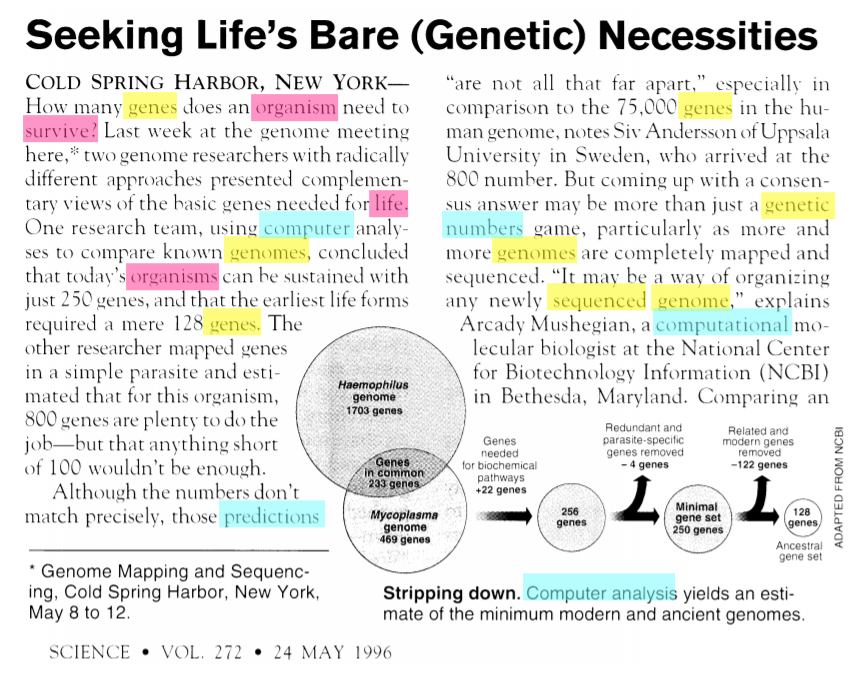
\includegraphics[scale = 0.30]{../plots/presentation/motivation.png}
	\end{figure}
\item Question at hand: how to assign colored words to topics?
\end{itemize}
\end{frame}

\begin{frame}
\frametitle{Topic Modeling: Motivation and Theory}
\framesubtitle{Notation and Terminology (I)}
\begin{itemize}
\item \textit{Words} $w$: instances of a vocabulary of $V$ unique \textit{terms}
\item \textit{Documents} $d \in \{1,\dots,D\}$: sequences of words of length $N_{d}$; $w_{d,n}$ denoting $n$-th word of document $d$
\item \textit{Corpus}: collection (or set) of $D$ documents
\item \textit{Topics} $k \in \{1,\dots,K\}$: latent thematic clusters within a text corpus; (implicit) representation of a corpus
\item \textit{Topic-word distributions} $\boldsymbol{\beta}$: probability distributions over words; $\boldsymbol{\beta}_k$ denoting the word distribution corresponding to the $k$-th topic
\end{itemize}
\end{frame}

\begin{frame}
\frametitle{Topic Modeling: Motivation and Theory}
\framesubtitle{Notation and Terminology (II)}
\begin{itemize}
\item \textit{Topic assignments} $\boldsymbol{z}_{d,n}$: assignment of $w_{d,n}$ to a specific topic $k \in \{1,\dots,K\}$; $\boldsymbol{\beta}_{d,n}$ representing the (assigned) word distribution for $w_{d,n}$
\item \textit{Topic proportions} $\boldsymbol{\theta}_d$: proportions of document $d$'s words assigned to each of the topics; $\sum_{k=1}^{K}\theta_{d,k}=1$, for all $d \in \{1,\dots,D\}$
\item \textit{Bag-of-word} assumption: only words themselves meaningful, unlike word order or grammar; equivalent to assuming \textit{exchangeability} \cite{aldous1985exchangeability}
\end{itemize}
\end{frame}

\begin{frame}
\frametitle{Topic Modeling: Motivation and Theory}
\framesubtitle{\textit{Latent Dirichlet Allocation} (LDA) (I)}
\begin{itemize}
\item First topic model with entirely probabilistic generating process: LDA \cite{blei2003latent}
\item Generative process for each document $d \in \{1,\dots,D\}$:
\item[] 
	\begin{enumerate}[{1)}]
	\item Draw topic proportions $\boldsymbol{\theta}_d \sim \text{Dir}_K(\boldsymbol{\alpha})$.
	\item For each word $n \in \{1,\dots,N_d\}$:
		\begin{enumerate}[{a)}]
		\item Draw a topic assignment $\boldsymbol{z}_{d,n} \sim \text{Multinomial}_K(\boldsymbol{\theta}_d)$.
		\item Draw a word $w_{d,n} \sim \text{Multinomial}_V(\boldsymbol{\beta}_{d,n})$.
	\end{enumerate}
\end{enumerate}
\item Graphical model representation of LDA: \cite{blei2003latent} 
	\begin{figure}[h!]
  	\centering
  	\hspace*{-1cm}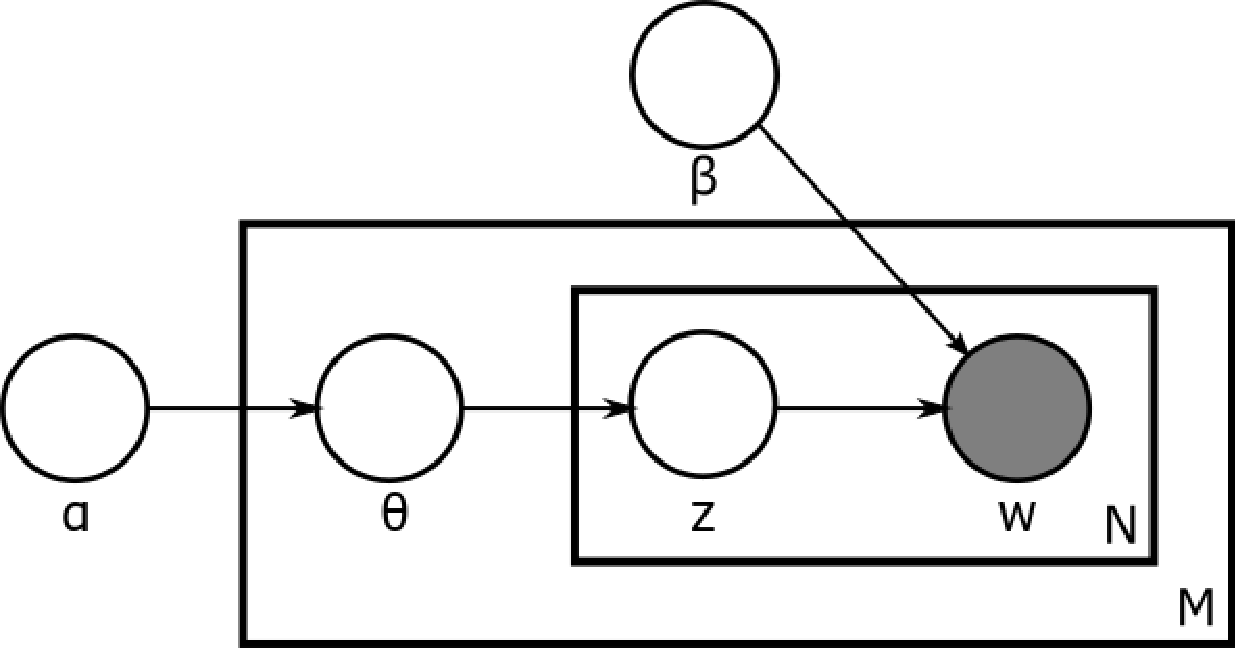
\includegraphics[scale = 0.3]{../plots/presentation/lda_graphical.pdf}
	\end{figure}
\end{itemize}
\end{frame}

\begin{frame}
\frametitle{Topic Modeling: Motivation and Theory}
\framesubtitle{\textit{Latent Dirichlet Allocation} (LDA) (II)}
\begin{itemize}
\vspace{-0.5cm}
\item Illustration of topic assignment for the words of a document: \cite{blei2012probabilistic}
	\vspace{-0.5cm}
	\begin{figure}[h!]
  	\centering
  	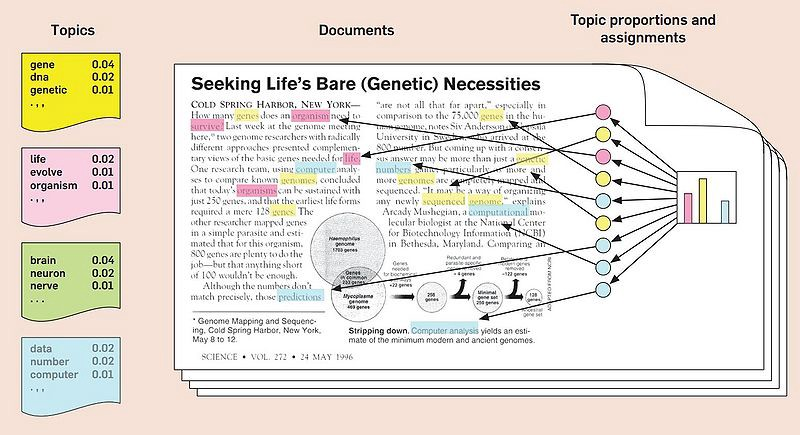
\includegraphics[scale = 0.4]{../plots/presentation/lda_topic_assignment.jpeg}
	\end{figure}
\end{itemize}
\end{frame}

\begin{frame}
\frametitle{Topic Modeling: Motivation and Theory}
\framesubtitle{\textit{Structural Topic Model} (STM)}
\begin{itemize}
\item Topic model that incorporates document-level metadata: 
\begin{itemize}
\item \textit{Topical prevalence} covariates $\boldsymbol{X}=[\boldsymbol{x_1}|\dots|\boldsymbol{x_D}]^T \in \mathbb{R}^{D \times P}$
\item Categorical \textit{topical content} variable $\boldsymbol{Y}\in \mathbb{R}^D$ with $A$ levels, i.e., $Y_d \in \{1,\dots,A\}$, for all $d \in \{1,\dots,D\}$
\end{itemize}
\item Generative process for each document $d \in \{1,\dots,D\}$:
\item[] 
\begin{enumerate}[{1)}]
\item Draw $\boldsymbol{\eta}_d \sim \mathcal{N}_{K-1}(\boldsymbol{\Gamma}^T\boldsymbol{x_d}^T, \boldsymbol{\Sigma})$, with $\eta_{d,K}=0$ for model identifiability.
\item Normalize $\boldsymbol{\eta}_d$, for all $k \in \{1,\dots,K\}: \theta_{d,k} = \frac{exp(\eta_{d,k})}{\sum_{j=1}^{K}exp(\eta_{d,j})}$.
\item For each word $n \in \{1,\dots,N_d\}$:
	\begin{enumerate}[{a)}]
    \item Draw topic assignment $\boldsymbol{z}_{d,n} \sim \text{Multinomial}_K(\boldsymbol{\theta}_d)$.
    \item If no topical content variable specified: $w_{d,n} \sim \text{Multinomial}_V(\boldsymbol{\beta}_{d,n})$. 
    \item[] Otherwise, determine document-specific word distributions $\boldsymbol{B_a} := [\boldsymbol{\beta}^a_1|\dots|\boldsymbol{\beta}^a_K]$ based on $Y_d=a$, for all topics $k \in \{1,\dots,K\}$; select $\boldsymbol{\beta}_{d,n}:=\boldsymbol{B_a}\boldsymbol{z}_{d,n}$; and draw word $w_{d,n} \sim \text{Multinomial}_V(\boldsymbol{\beta}_{d,n})$.
	\end{enumerate}
\end{enumerate}
\end{itemize}
\end{frame}

\begin{frame}
\frametitle{Topic Modeling: Motivation and Theory}
\framesubtitle{Graphical Model of the STM}
\begin{itemize}
\item Visualization of the generative process again through graphical model \cite{roberts2016model}:
\begin{figure}[h!]
\centering
\hspace*{-1cm}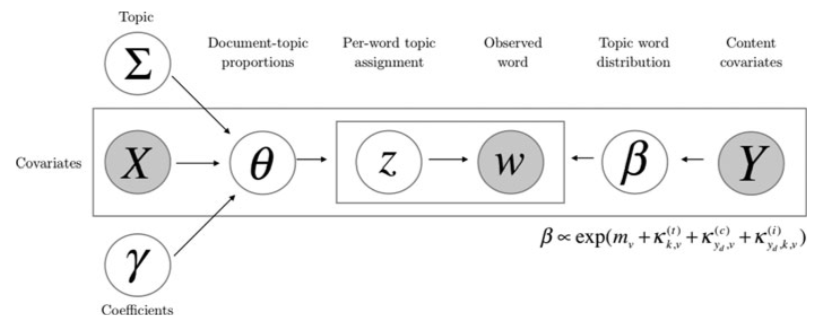
\includegraphics[scale = 0.4]{../plots/presentation/stm_graphical.png}
\end{figure}
\end{itemize}
\end{frame}

\begin{frame}
\frametitle{Topic Modeling: Motivation and Theory}
\framesubtitle{\textit{Inference and Parameter Estimation}}
\begin{itemize}
\vspace{-0.5cm}
\item (Hierarchical) Bayesian model $\Rightarrow$ exact inference impossible due to marginal distributions in the denominator of posterior distribution $p$
\item Variational inference: positing a simple distribution family $q$ for latent variables $\boldsymbol{\theta}$ and $\boldsymbol{z}$
\item Mean-field variational inference: positing full factorizability of approximating posterior $q$, i.e., $q(\boldsymbol{\theta}, \boldsymbol{z})=q(\boldsymbol{\theta})q(\boldsymbol{z})$
\item Then: minimizing Kullback-Leibler divergence between $q$ and $p$
\item STM uses a mean-field variational EM algorithm:
\begin{itemize}
\item E-step: update posterior distributions of latent variables $\boldsymbol{\theta}$ and $\boldsymbol{z}$
\item M-step: update model parameters $\boldsymbol{\Gamma}$, $\boldsymbol{\Sigma}$, and - if present - topical content parameters
\end{itemize}
\end{itemize}
\end{frame}

\section{Data}
\begin{frame}
\frametitle{Data}
\framesubtitle{Data Collection (I)}
\begin{itemize}
\item MP-level data: from \url{www.bundestag.de/abgeordnete} using Python's \textit{BeautifulSoup} and a \textit{selenium web driver} \cite{van1995python} \cite{richardson2007beautiful}
\item[] 
	\begin{figure}[h!]
  	\centering
  	
\includegraphics[scale = 0.30]{../plots/presentation/amthor.png}
	\end{figure}
\item Twitter profiles: from official party homepages
\item Socioeconomic data and 2017 German federal election results: from \url{www.bundeswahlleiter.de}
\end{itemize}
\end{frame}

\begin{frame}
\frametitle{Data}
\framesubtitle{Data Collection (II)}
\begin{itemize}
\item Tweets (and further Twitter features): via the official Twitter API using Python's \textit{tweepy} library\cite{roesslein2020tweepy}
\item Monthly tweets (after dropping MPs without electoral district) for our period of analysis, September 24, 2017 through April 24, 2020:
	\begin{figure}[h!]
  	\centering
  	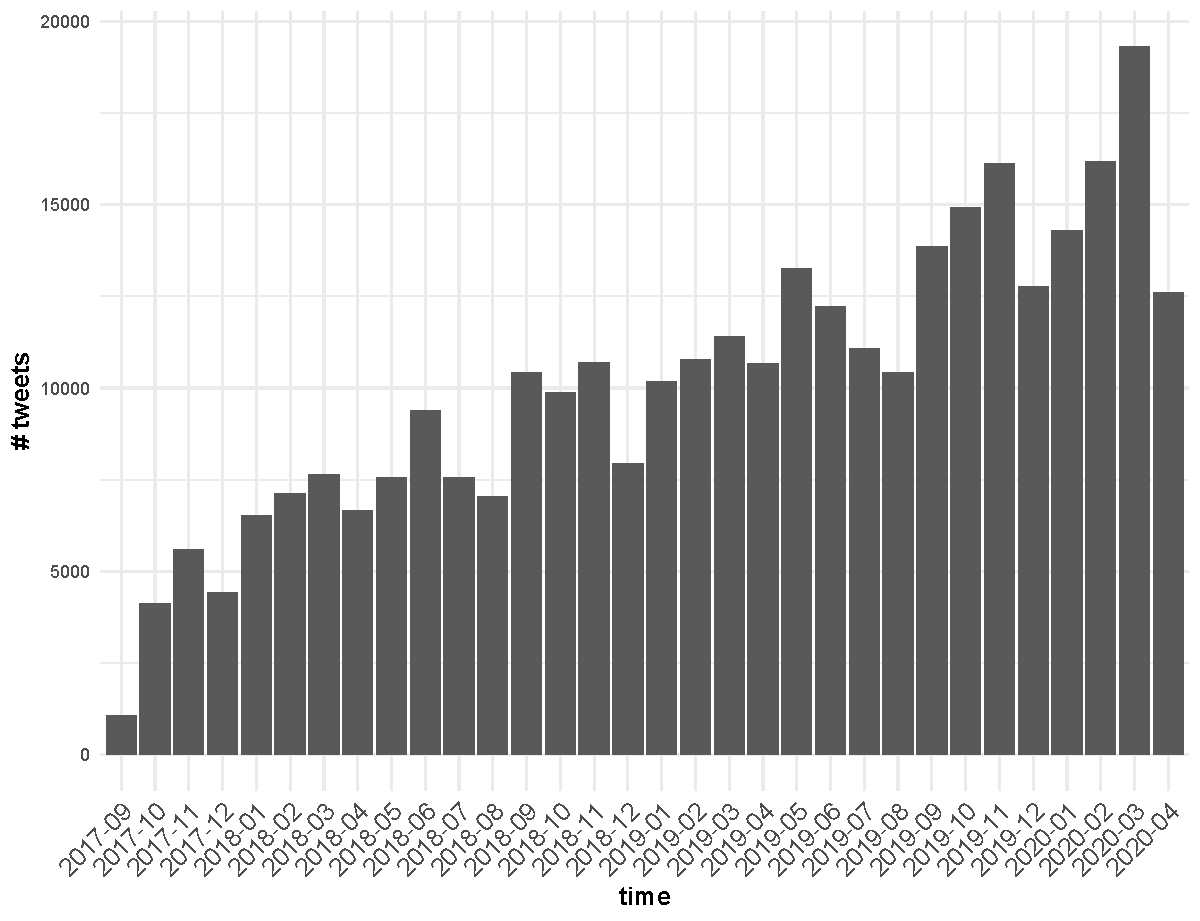
\includegraphics[scale = 0.30]{../plots/3/monthly_tweets.pdf}
	\end{figure}
\item In the following: grouping each MP's tweets on a monthly basis
\end{itemize}
\end{frame}

\begin{frame}
\frametitle{Data}
\framesubtitle{Data Preprocessing}
\begin{itemize}
\item Preprocessing: in R \cite{R}, using the \textit{quanteda} package \cite{quanteda}
\item Transcription of German umlauts (e.g. \"a $\rightarrow$ a) and ligature (\ss $\rightarrow$ ss)
\item Removal of hyphens: relevant for compound words (e.g., \textit{Corona-Krise} vs \textit{Coronakrise})
\item Transformation of text data into document-feature matrix (DFM); conversion to lowercase; removal of stopwords, units (\textit{kg}, \textit{uhr}), interjections (\textit{aaahhh}, \textit{ufff}), etc.
\item Word stemming, i.e., cutting off word endings (e.g., \textit{politisch} $\rightarrow$ \textit{polit}) \cite{lucas2015computer}
\end{itemize}
\end{frame}

\section{Model Selection and Global Characteristics}
\begin{frame}
\frametitle{Model Selection and Global Characteristics}
\framesubtitle{Model Selection}
\begin{itemize}
\item Model evaluation metrics for hyperparameter $K$ (number of topics):
	\begin{figure}[h!]
  	\centering
  	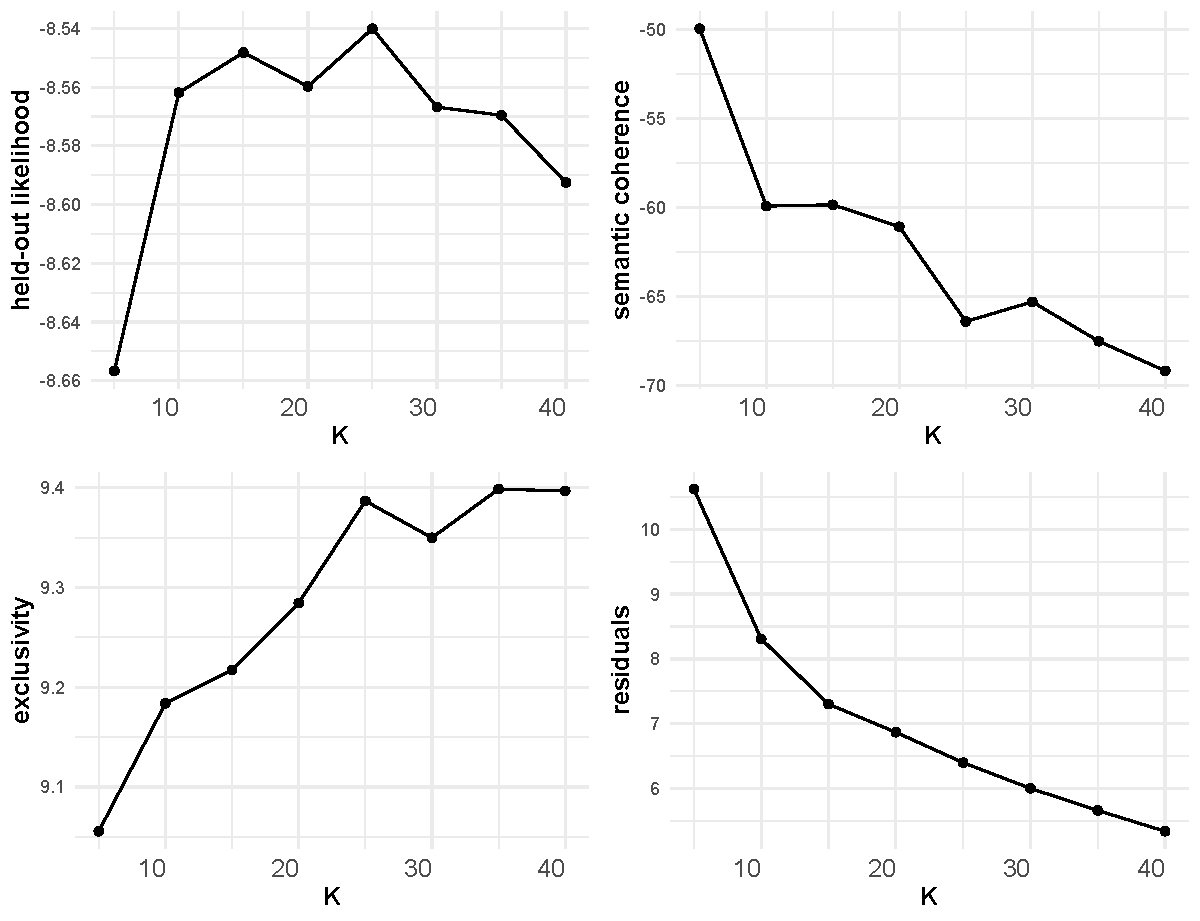
\includegraphics[scale = 0.30]{../plots/4_1/searchK.pdf}
	\end{figure}
\item "Best" trade-off: $K=15$
\end{itemize}
\end{frame}

\begin{frame}
\frametitle{Model Selection and Global Characteristics}
\framesubtitle{Labeling (I)}
\begin{itemize}
\item Three-step procedure for labeling
\item First step: top words for different weighting methodologies
\begin{table}[h!]
\centering
\resizebox{8cm}{!}{%
\begin{tabular}{|l|}
\hline
\textit{Topic 1 Top Words:}\\
 	 \textbf{Highest Prob:} buerg, link, merkel, frau, sich \\
 	 \textbf{FREX:} altpartei, islam, linksextremist, asylbewerb, linksextrem \\
 	 \textbf{Lift:} eitan, 22jaehrig, abdelsamad, abgehalftert, afdforder \\
 	 \textbf{Score:} altpartei, linksextremist, frauenkongress, islamist, boehring \\
\hline
\textit{Topic 3 Top Words:}\\
 	 \textbf{Highest Prob:} brauch, wichtig, leid, dank, klar \\
 	 \textbf{FREX:} emissionshandel, soli, marktwirtschaft, feedback, co2steu \\
 	 \textbf{Lift:} aequivalenz, altersvorsorgeprodukt, bildungsqualitaet, co2limit, co2meng \\
 	 \textbf{Score:} emissionshandel, co2limit, basisrent, euet, technologieoff \\
\hline
\textit{Topic 4 Top Words:}\\
 	 \textbf{Highest Prob:} sozial, miet, kind, arbeit, brauch \\
 	 \textbf{FREX:} mindestlohn, miet, wohnungsbau, mieterinn, loehn \\
 	 \textbf{Lift:} auseinanderfaellt, baugipfel, bestandsmiet, billigflieg, binnennachfrag \\
 	 \textbf{Score:} miet, mieterinn, mietendeckel, grundsicher, bezahlbar \\
\hline
\textit{Topic 6 Top Words:}\\
 	 \textbf{Highest Prob:} gruen, klimaschutz, brauch, klar, euro \\
 	 \textbf{FREX:} fossil, erneuerbar, kohleausstieg, verkehrsminist, verkehrsw \\
 	 \textbf{Lift:} abgasbetrug, abgebaggert, abschalteinricht, abschaltet, ammoniak \\ 
 	 \textbf{Score:} erneuerbar, fossil, zdebel, verkehrsminist, klimaschutz \\
\hline
\end{tabular}%
}
\end{table}
\end{itemize}
\end{frame}

\begin{frame}
\frametitle{Model Selection and Global Characteristics}
\framesubtitle{Labeling (II)}
\begin{itemize}
\item Word cloud of \textbf{Highest Prob} top words (for topic 1):
	\begin{figure}[h!]
  	\centering
  	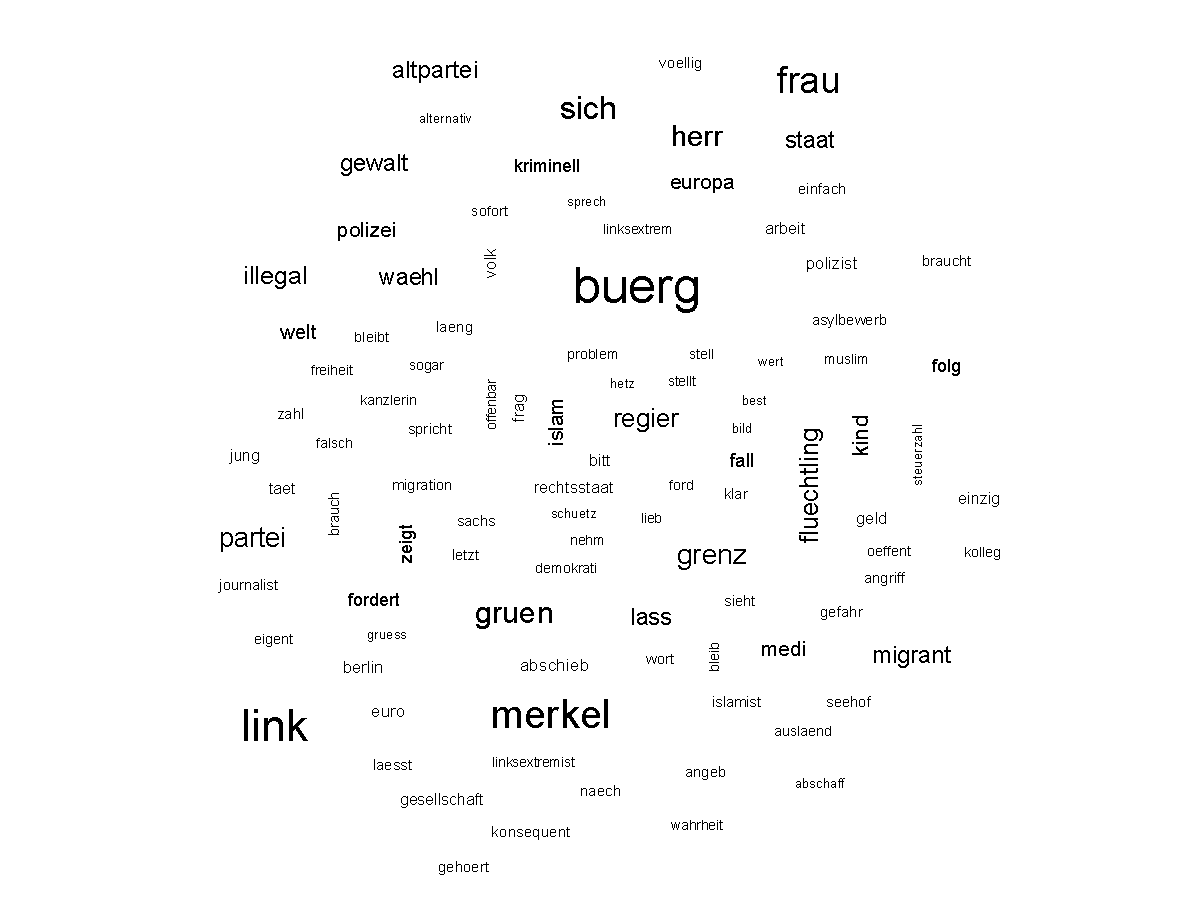
\includegraphics[scale = 0.40]{../plots/4_2/t1_wordcloud.pdf}
	\end{figure}
\item Word size corresponding to word frequency in topic 1
\end{itemize}
\end{frame}

\begin{frame}
\frametitle{Model Selection and Global Characteristics}
\framesubtitle{Labeling (III)}
\begin{itemize}
\item Second step: looking at documents (i.e., original tweets) with highest proportion of topic 1
	\begin{figure}[h!]
  	\centering
  	
\includegraphics[scale = 0.40]{../plots/presentation/martin_hess_topic1.png}
	\end{figure}
\end{itemize}
\end{frame}

\begin{frame}
\frametitle{Model Selection and Global Characteristics}
\framesubtitle{Labeling (IV)}
\begin{itemize}
\item Third step: assigning labels
\begin{table}[h!]
	\centering
	\resizebox{5cm}{!}{%
	\begin{tabular}{|l|l|}
	\hline
	Topic 1  & Right/Nationalist    \\ \hline
	Topic 2  & Miscellaneous 1      \\ \hline
	Topic 3  & Climate Economics    \\ \hline
	Topic 4  & Social/Housing       \\ \hline
	Topic 5  & Digital/Future       \\ \hline
	Topic 6  & Climate Protection   \\ \hline
	Topic 7  & Europe               \\ \hline
	Topic 8  & Corona               \\ \hline
	Topic 9  & Left/Anti-war        \\ \hline
	Topic 10 & Twitter/Politics 1   \\ \hline
	Topic 11 & Twitter/Politics 2   \\ \hline
	Topic 12 & Miscellaneous 2      \\ \hline
	Topic 13 & Twitter/Politics 3   \\ \hline
	Topic 14 & Right-wing Extremism \\ \hline
	Topic 15 & Society/Solidarity   \\ \hline
	\end{tabular}
	}
\end{table}
\end{itemize}
\end{frame}

\begin{frame}
\frametitle{Model Selection and Global Characteristics}
\framesubtitle{Global Topic Proportions}
\begin{itemize}
\item Illustration of \textbf{global} topic proportions:
	\begin{figure}[h!]
  	\centering
  	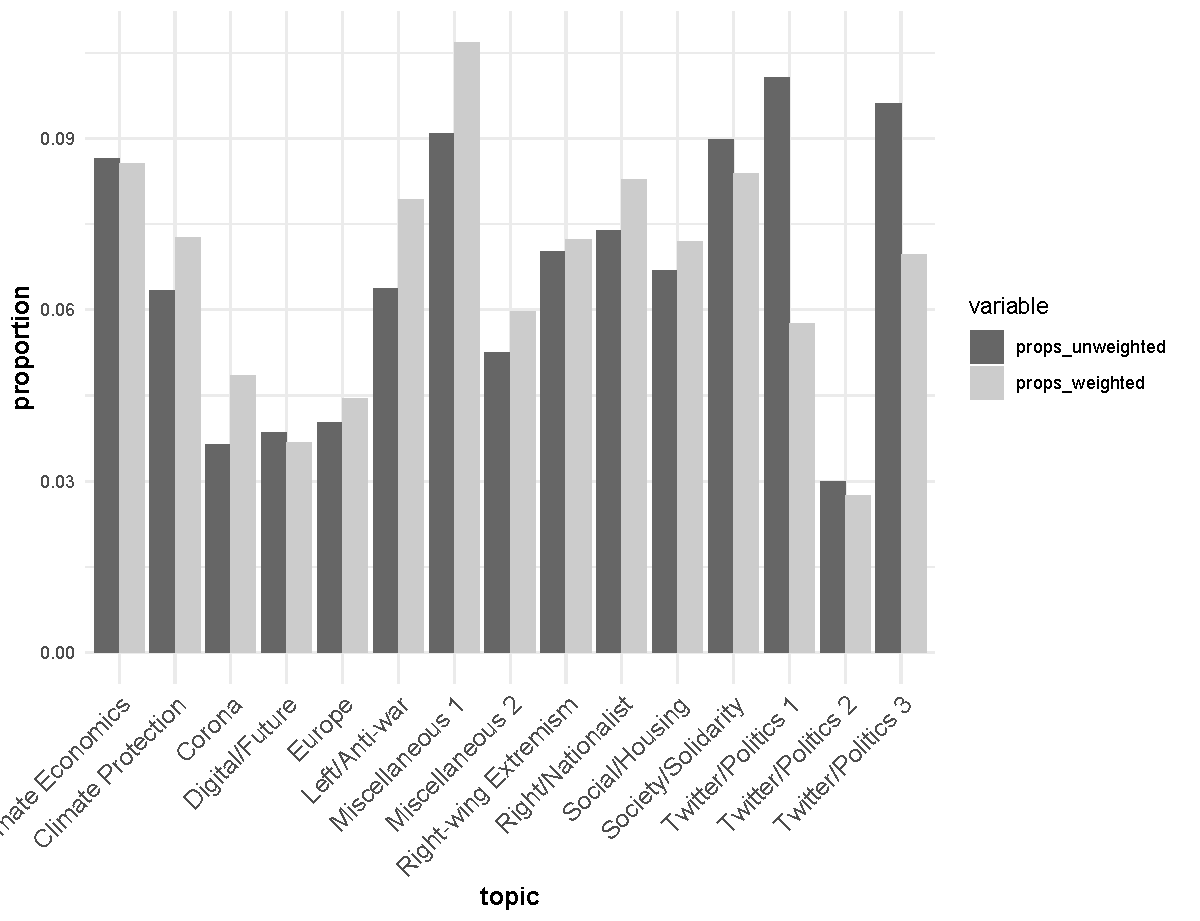
\includegraphics[scale = 0.40]{../plots/4_3/global_thetas.pdf}
	\end{figure}
\end{itemize}
\end{frame}

\begin{frame}
\frametitle{Model Selection and Global Characteristics}
\framesubtitle{Global Topic Correlations}
\begin{itemize}
\item Vocabulary overlap (left) and topic correlations (right):
\begin{figure}[h!]
  \resizebox{14cm}{!}{%	
  \centering
  \begin{subfigure}[b]{0.4\linewidth}
    \hspace*{-0.7cm}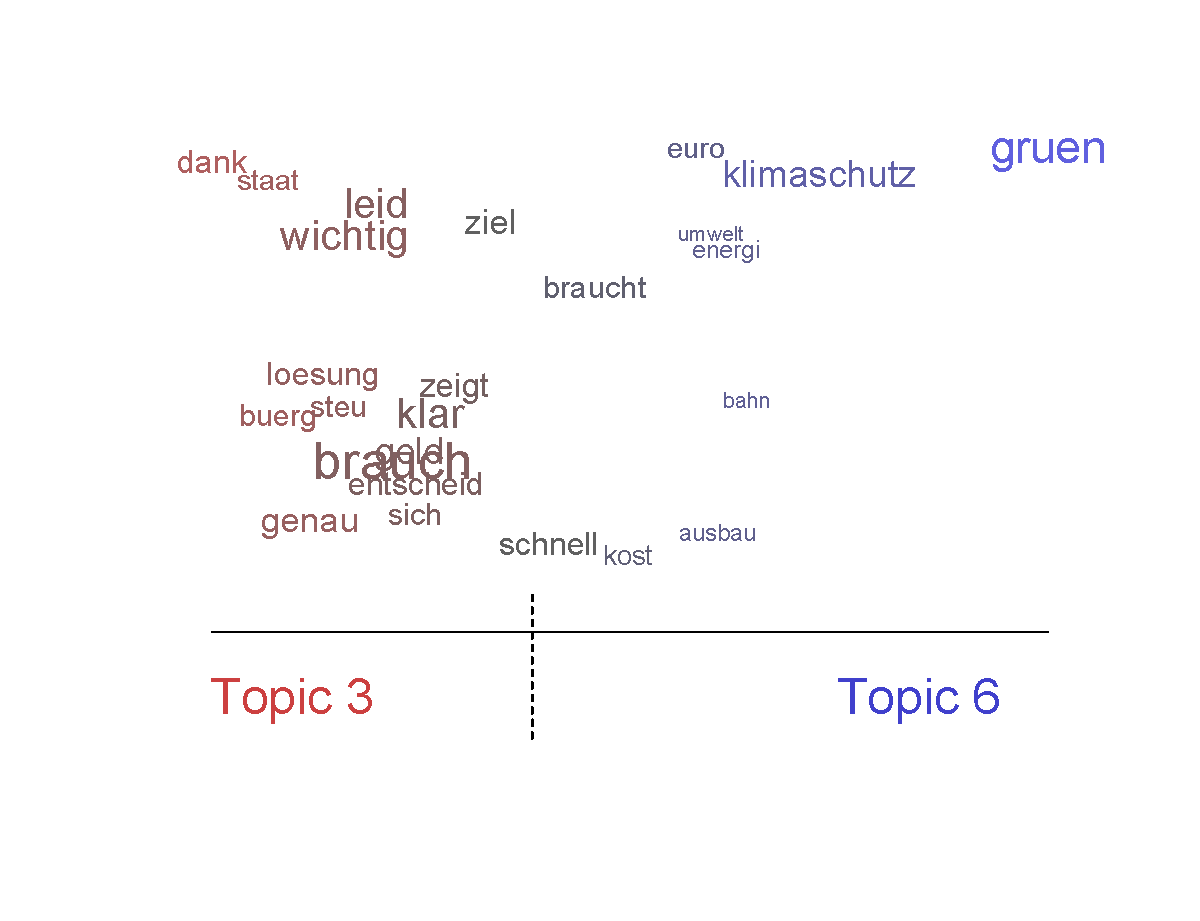
\includegraphics[width=\linewidth]{../plots/4_3/vocabulary_comparison.pdf}
  \end{subfigure}
  \begin{subfigure}[b]{0.4\linewidth}
    \hspace*{-1.1cm}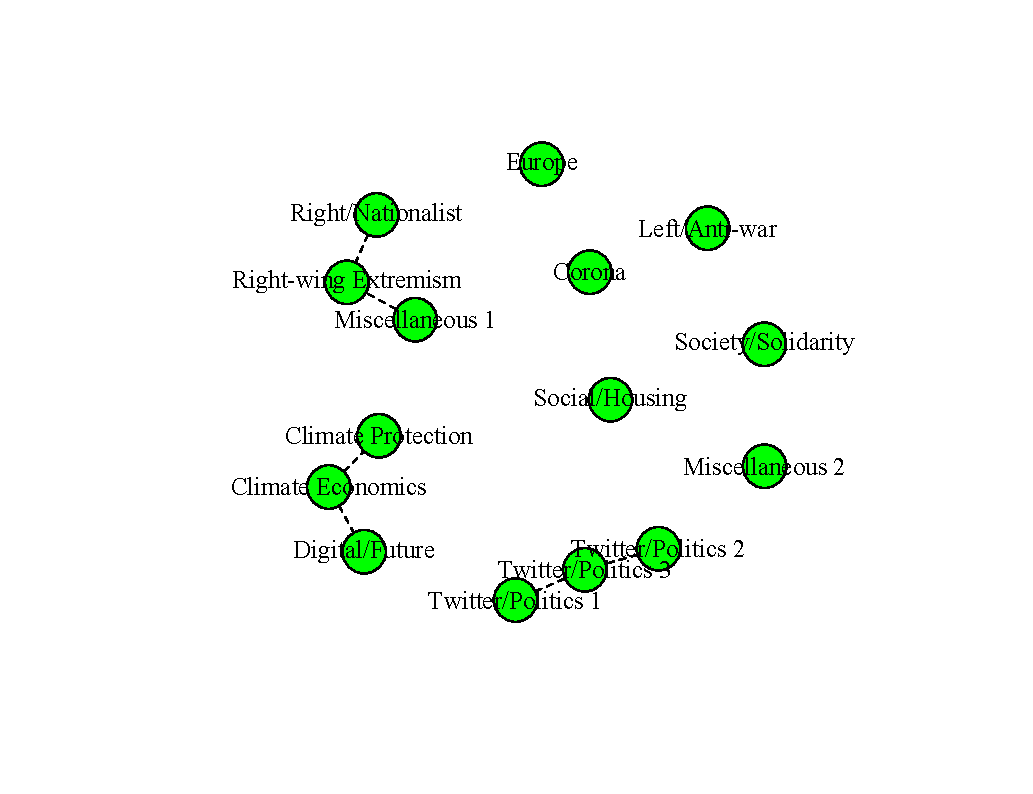
\includegraphics[width=\linewidth]{../plots/4_3/topic_correlations_map.pdf}
  \end{subfigure}
  }
\end{figure}		
\end{itemize}
\end{frame}

\section{Covariate-level Topic Analysis}
\begin{frame}
\frametitle{Covariate-level Topic Analysis}
\framesubtitle{Overview}
\begin{itemize}
\item Explore estimated topical structure with respect to different dimensions, e.g.\ membership in political party, time, $\dots$
\item Precisely: examine relationship between document-level prevalence covariates $\boldsymbol{x}_d$ and topic proportions $\boldsymbol{\theta}_d$
\item Natural idea: regress topic proportions on prevalence covariates
\item Problem: $\boldsymbol{\theta}_d$ is \textit{latent} variable and has to be estimated itself!
\item In following two approaches to address this problem:
\begin{enumerate}
\item Regression that takes into account uncertainty about $\boldsymbol{\theta}_d$: perform sampling technique known as "method of composition" in social sciences
\item Direct assessment of STM output via logistic normal distribution with estimated topical prevalence parameters $\hat{\boldsymbol{\Gamma}}$ and $\hat{\boldsymbol{\Sigma}}$
\end{enumerate}
\end{itemize}
\end{frame}

\begin{frame}
\frametitle{Covariate-level Topic Analysis}
\framesubtitle{Method of Composition}
\begin{itemize}
\item Let $\boldsymbol{\theta}_{(k)}:=(\theta_{1,k}, \dots, \theta_{D,k})^T \in [0,1]^{D}$ denote proportion of $k$-th topic for all $D$ documents
\item Method of Composition (repeat $m$ times):
\begin{enumerate}
\item Sample $\boldsymbol{\theta}^*_{(k)}$ from (variational) posterior of $\boldsymbol{\theta}_{(k)}$ estimated by STM
\item Run regression model with response $\boldsymbol{\theta}^*_{(k)}$ and covariates $\boldsymbol{X}$ to obtain estimate $\hat{\boldsymbol{\xi}}^*$ of regression coefficients $\boldsymbol{\xi}^*$ and covariance of $\hat{\boldsymbol{\xi}}^*$, $\hat{\boldsymbol{V}}^*_{\xi}$
\item Sample $\tilde{\boldsymbol{\xi}}^*$ from $F(\hat{\boldsymbol{\xi}}^*, \hat{\boldsymbol{V}}^*_{\xi})$, where $F$ is (asymptotic) distribution of $\hat{\boldsymbol{\xi}}^*$
\end{enumerate}
\item Idea: samples $\tilde{\boldsymbol{\xi}}^*$ take into account uncertainty in $\boldsymbol{\theta}_{(k)}$
\item Visualization of topic-metadata relationship: For observation $\boldsymbol{x}_{\text{pred}}$, plot $\boldsymbol{x}_{\text{pred}}$ vs. predicted response with $\boldsymbol{x}_{\text{pred}}^T \tilde{\boldsymbol{\xi}}^*$ as linear predictor
\end{itemize}
\end{frame}

\begin{frame}
\frametitle{Covariate-level Topic Analysis}
\framesubtitle{Method of Composition: Problems}
Several problems with method of composition:
\begin{enumerate}
\item In STM, regression model in step 2 is OLS; however OLS not appropriate to model (sampled) proportions in open unit interval
\item Mixing of Bayesian and frequentist approach questionable:
\begin{itemize}
\item From Bayesian perspective, $\tilde{\boldsymbol{\xi}}^*$ can only be considered sample from posterior of $\boldsymbol{\xi}$ in certain Bayesian regression models with questionable (uniform) prior assumptions
\item Using $\boldsymbol{x}_{\text{pred}}^T \tilde{\boldsymbol{\xi}}^*$  as linear predictor does \textit{not} yield sample of posterior predictive distribution
\end{itemize}
\item Separate modeling of topic proportions neglects dependence of different topics among each other
\end{enumerate}
\end{frame}

\begin{frame}
\frametitle{Covariate-level Topic Analysis}
\begin{center}
Problem 1: OLS Regression
\end{center}
\end{frame}

\begin{frame}
\frametitle{Covariate-level Topic Analysis}
\framesubtitle{Method of Composition: Implementation within \textit{stm}}
\begin{itemize}
\item Problem: OLS regression not suitable for (sampled) proportions, which are restricted to interval (0,1)
\item Estimated relationship between proportions and prevalence covariates might even involve negative proportions:
\end{itemize}
\frametitle{Covariate-level Topic Analysis}
\framesubtitle{Method of Composition: Usage within R Package \textit{stm}}
  \begin{figure}[h!]
  \centering
  \captionsetup{justification=centering,margin=2cm}
  \begin{subfigure}[b]{0.4\linewidth}
    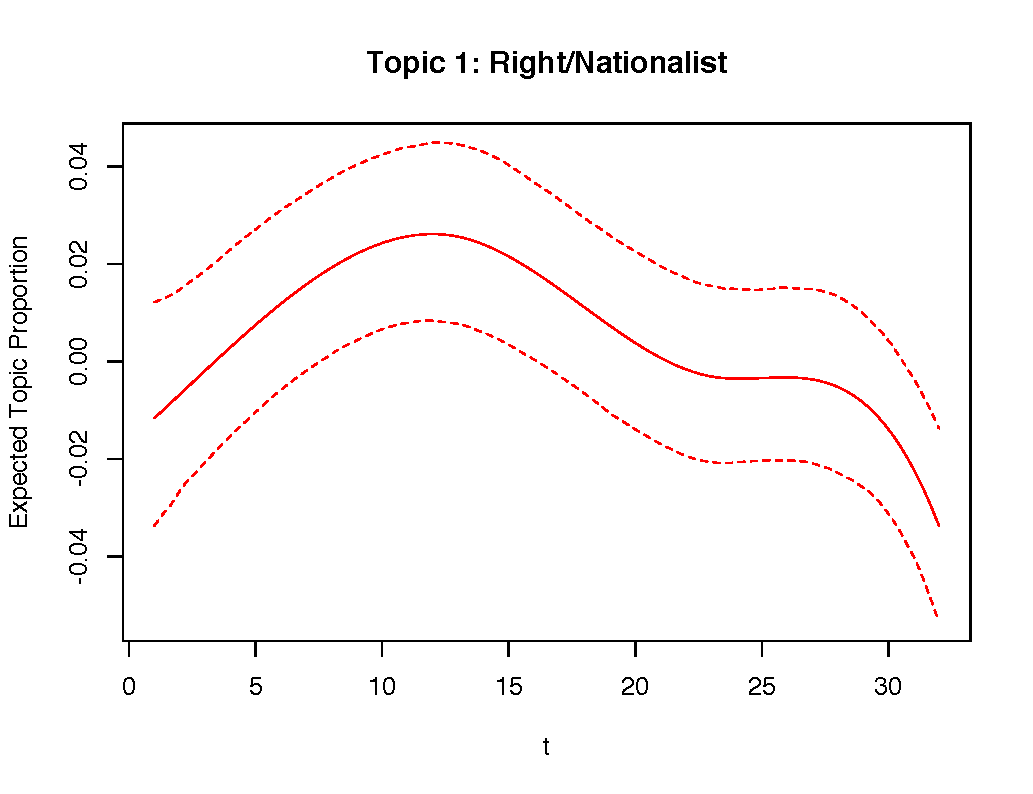
\includegraphics[width=\linewidth]{../plots/presentation/estEffect_topic1.pdf}
  \end{subfigure}
  \begin{subfigure}[b]{0.4\linewidth}
    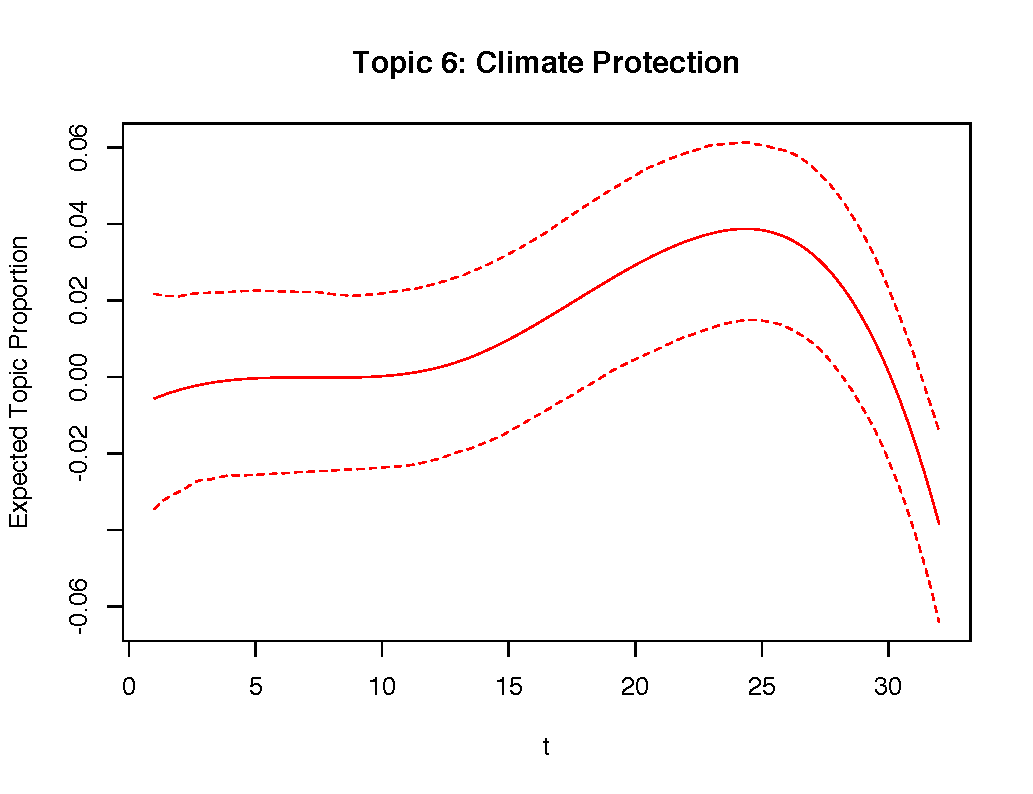
\includegraphics[width=\linewidth]{../plots/presentation/estEffect_topic6.pdf}
  \end{subfigure}
\end{figure}
\end{frame}

\begin{frame}
\frametitle{Covariate-level Topic Analysis}
\framesubtitle{Method of Composition: Extension of existing approach}
\begin{itemize}
\item Instead of OLS regression, we can use a beta regression or a quasibinomial GLM (both with logit-link) to adequately model proportions
\end{itemize}
\begin{figure}[h!]
  \centering
  \captionsetup{justification=centering,margin=2cm}
  \begin{subfigure}[b]{0.4\linewidth}
    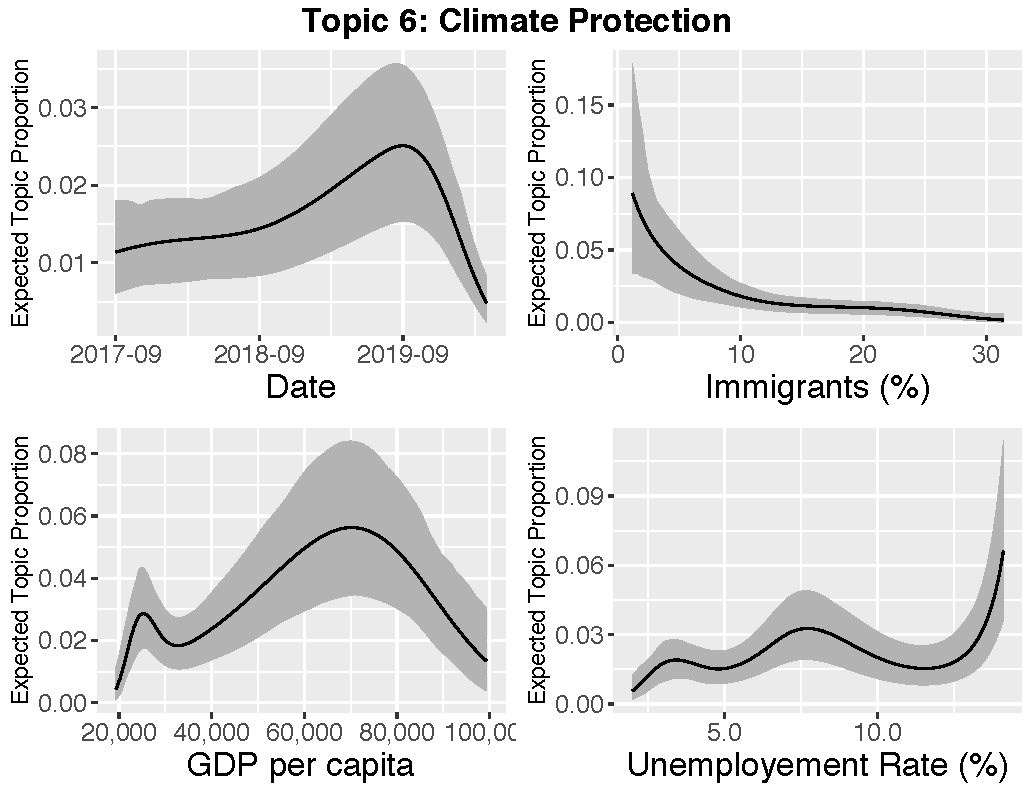
\includegraphics[width=\linewidth]{../plots/presentation/quasi_t6_cont.pdf}
  \end{subfigure}
  \begin{subfigure}[b]{0.4\linewidth}
    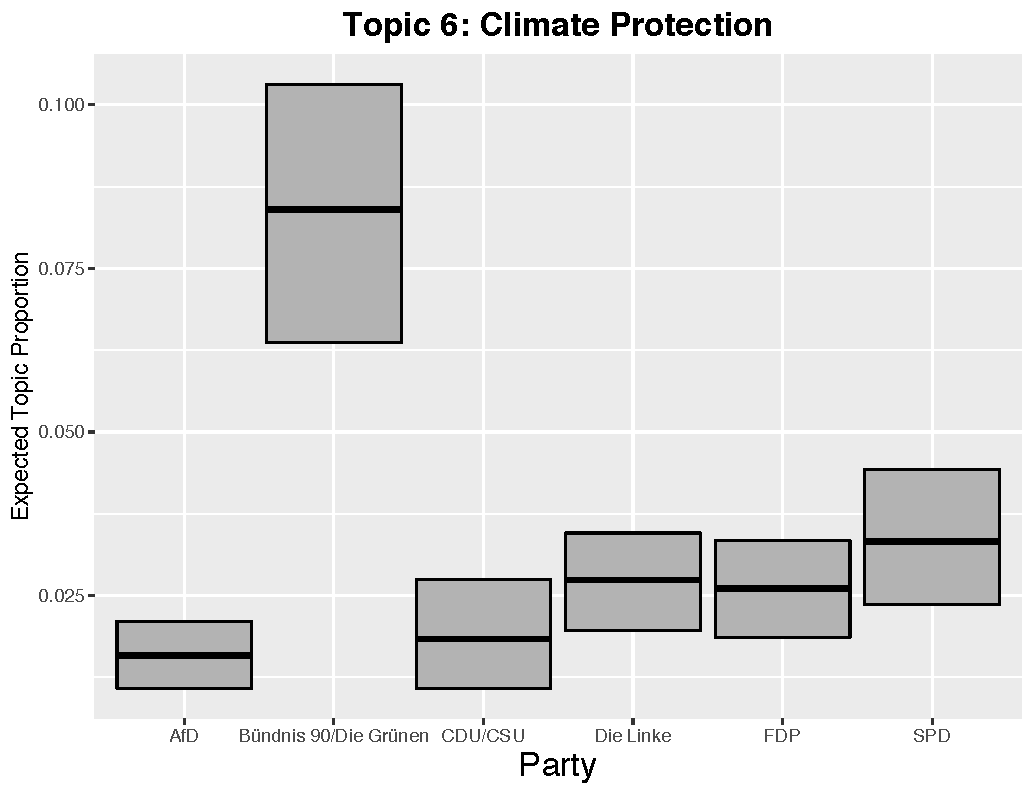
\includegraphics[width=\linewidth]{../plots/presentation/quasi_t6_cat.pdf}
  \end{subfigure}
\end{figure}
\end{frame}

\begin{frame}
\frametitle{Covariate-level Topic Analysis}
\begin{center}
Problem 2: Mixing of Bayesian and Frequentist Approach
\end{center}
\end{frame}

\begin{frame}
\frametitle{Covariate-level Topic Analysis}
\framesubtitle{Mixing of Bayesian and Frequentist Approach}
\begin{itemize}
\item Regression within of method of composition is \textit{frequentist} regression
\item However, in STM $\tilde{\boldsymbol{\xi}}^*$ considered samples from (marginal, i.e., integrated over latent topic proportions) posterior of regression coefficients; only true by assuming uniform priors for $\boldsymbol{\xi}$
\item Caution: uncertainty from previous plots with respect to prediction of mean $\Rightarrow$ does \textit{not} reflect variation of topic proportions in data!
\item Better idea: fully Bayesian approach with more realistic priors and sampling from posterior predictive distribution to reflect variation of data
\end{itemize}
\end{frame}

\begin{frame}
\frametitle{Covariate-level Topic Analysis}
\framesubtitle{Fully Bayesian Approach: Idea}
\begin{itemize}
\item Idea: \textit{explicitly} perform Bayesian regression in second step of each iteration of method of composition
\item Modeling via beta regression (with normal priors centered around zero) in order to model proportions in $(0,1)$
\item Visualization: Sample proportions from posterior predictive distribution at end of each step of method of composition (i.e., conditioning on previously sampled $\boldsymbol{\theta}_{(k)}^*$) with covariate values $\boldsymbol{x}_{\text{pred}}$
\end{itemize}
\end{frame}

\begin{frame}
\frametitle{Covariate-level Topic Analysis}
\framesubtitle{Fully Bayesian Approach: Results}
\begin{itemize}
\item Predicted (empirical) mean mostly in line with results from previous analysis
\item Uncertainty now w.r.t.\ variation of topic proportions in data
\item Observed variation for topic proportions corresponds well to variation according to predictive posterior
\end{itemize}
\begin{figure}[h!]
  \centering
  \captionsetup{justification=centering}
  \begin{subfigure}[b]{0.4\linewidth}
    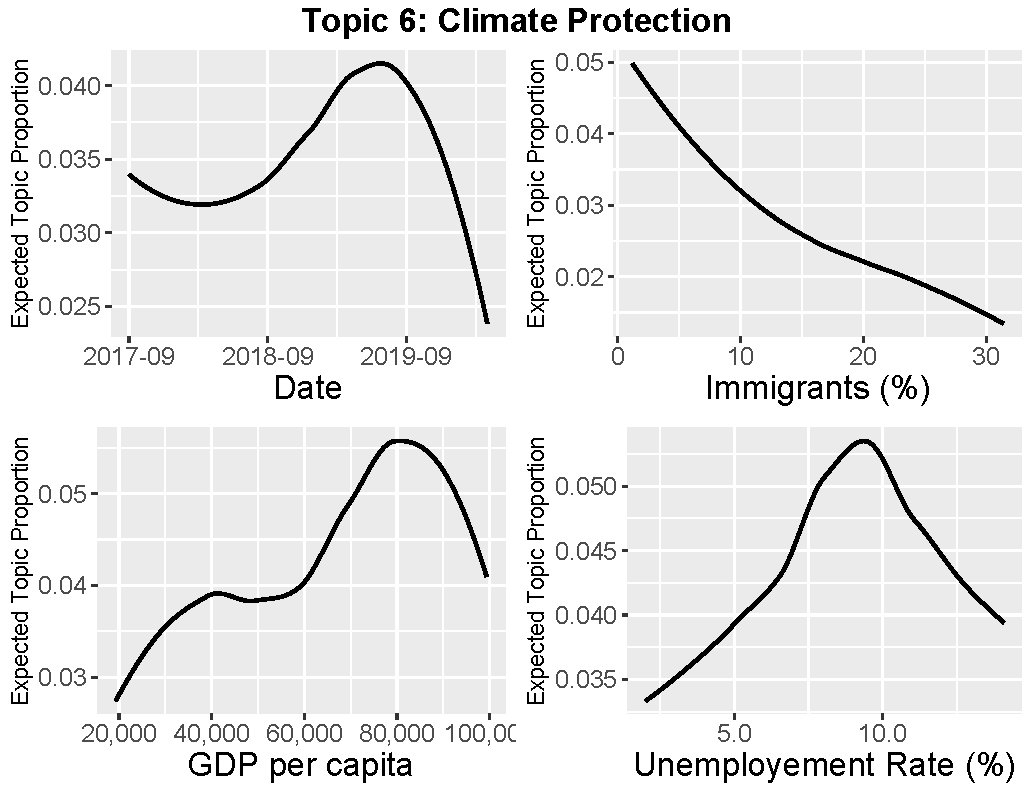
\includegraphics[width=\linewidth]{../plots/presentation/stanbeta_t6_without_credible.pdf}
  \end{subfigure}
  \begin{subfigure}[b]{0.4\linewidth}
    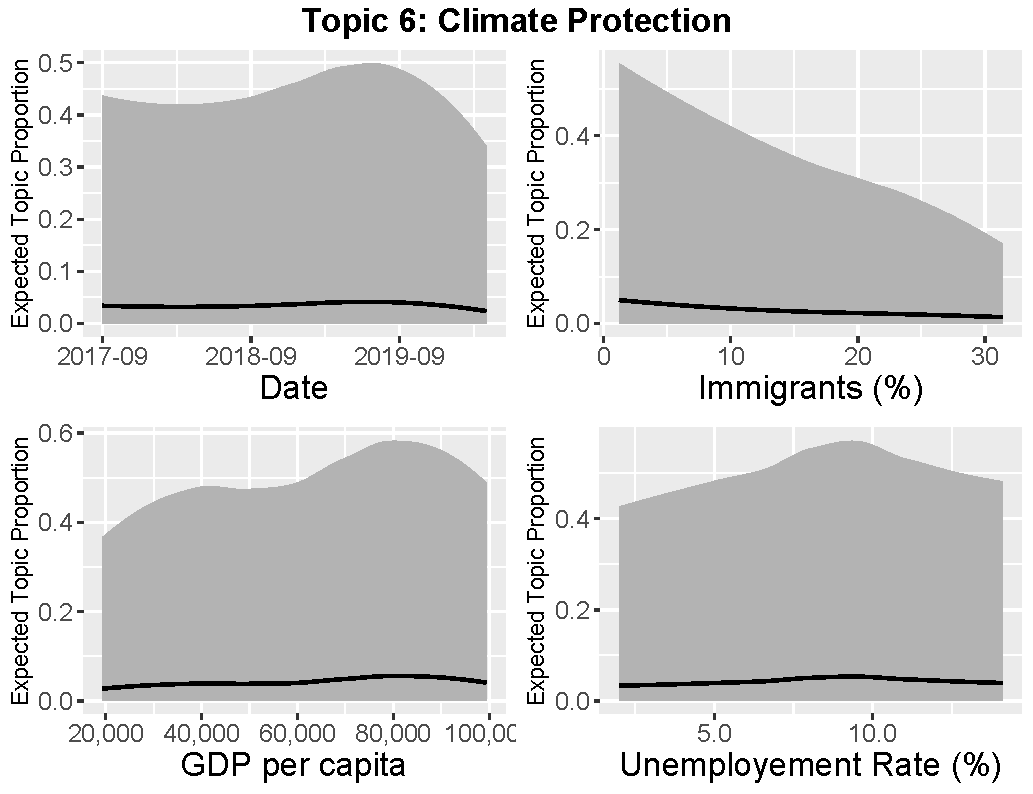
\includegraphics[width=\linewidth]{../plots/presentation/stanbeta_t6_with_credible.pdf}
  \end{subfigure}
\end{figure}
\end{frame}

\begin{frame}
\frametitle{Covariate-level Topic Analysis}
\begin{center}
Problem 3: Univariate Modeling of Topic Proportions
\end{center}
\end{frame}

\begin{frame}
\frametitle{Covariate-level Topic Analysis}
\framesubtitle{Approach to Multivariate Modeling of Proportions (I)}
\begin{itemize}
\item Remember, by assumption: $\boldsymbol{\theta}_d \sim \text{LogisticNormal}(\boldsymbol{\Gamma}^T\boldsymbol{x}_d^T, \boldsymbol{\Sigma})$
\item Logistic normal distribution assumes high dependence among individual components $\Rightarrow$ not fully taken into account in univariate modeling via, e.g., the beta distribution
\item Inference within STM involves finding estimates $\hat{\boldsymbol{\Gamma}}$ and $\hat{\boldsymbol{\Sigma}}$ $\Rightarrow$ Idea: plug estimates into logistic normal distribution
\item For given covariate value $\boldsymbol{x}_{\text{pred}}$, obtain topic proportion as $\boldsymbol{\theta}^*_d \sim \text{LogisticNormal}(\hat{\boldsymbol{\Gamma}}^T\boldsymbol{x}_{\text{pred}}^T, \hat{\boldsymbol{\Sigma}})$
\end{itemize}
\end{frame}

\begin{frame}
\frametitle{Covariate-level Topic Analysis}
\framesubtitle{Approach to Multivariate Modeling of Proportions (II)}
\begin{itemize}
\item Plugging in $\boldsymbol{\Gamma}$ and $\hat{\boldsymbol{\Sigma}}$ is "na{\"i}ve" method: ideally sample prevalence parameters from their posterior $\Rightarrow$ would yield higher variation
\item However, not easily possible $\Rightarrow$ should be addressed in future implementations
\end{itemize}
\begin{figure}[h!]
  \centering
  \captionsetup{justification=centering}
  \begin{subfigure}[b]{0.4\linewidth}
    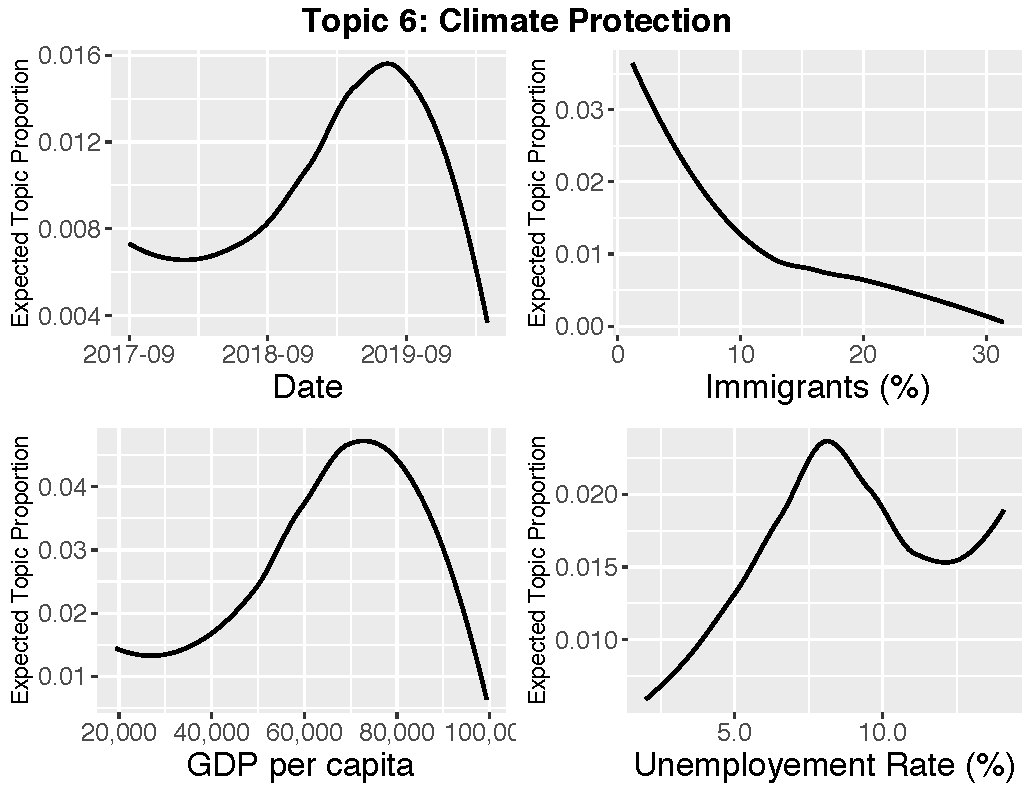
\includegraphics[width=\linewidth]{../plots/presentation/direct_t6_without_credible.pdf}
  \end{subfigure}
  \begin{subfigure}[b]{0.4\linewidth}
    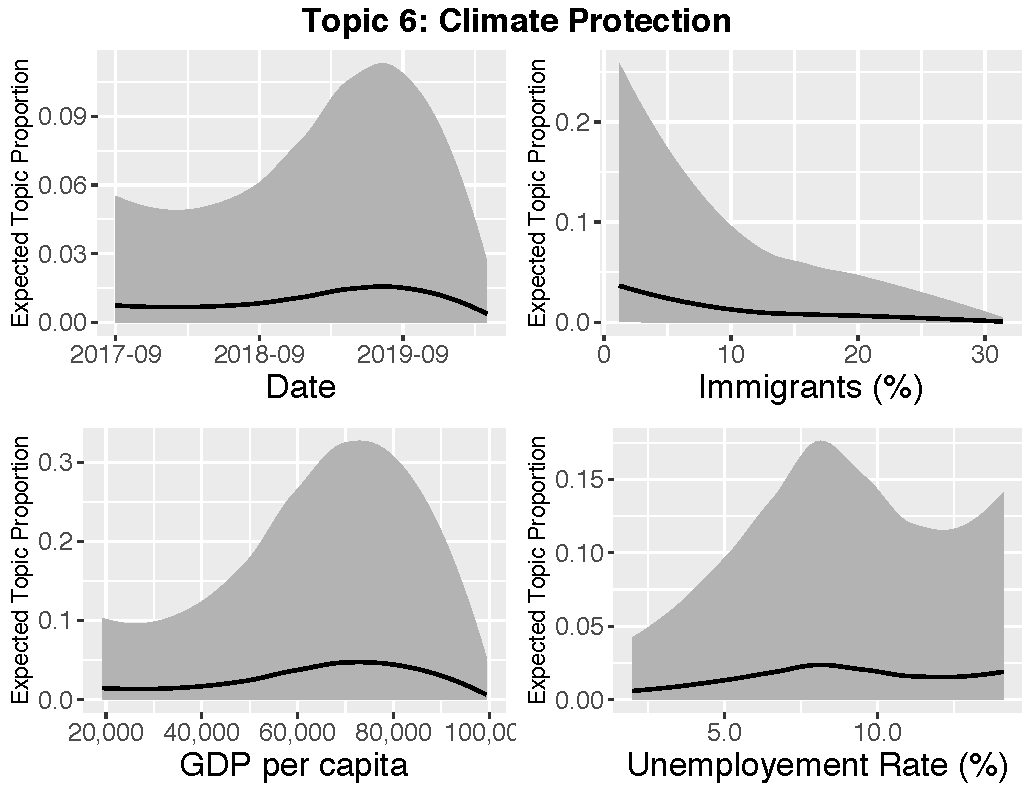
\includegraphics[width=\linewidth]{../plots/presentation/direct_t6_with_credible.pdf}
  \end{subfigure}
\end{figure}
\end{frame}

\section{Causal Inference}
\begin{frame}
\frametitle{Causal Inference}
\framesubtitle{Correlation vs. Causality (I)}
	\begin{figure}[h!]
  	\centering
  	
\includegraphics[scale = 0.60]{../plots/presentation/correlation_causality.png}
	\end{figure}
\end{frame}

\begin{frame}
\frametitle{Causal Inference}
\framesubtitle{Correlation vs. Causality (II)}
\begin{itemize}
\item In previous section: assessment of relationship between metadata and topic proportions
\item Framework to be used to \textit{explore} topics with respect to different dimensions
\item In particular, \textit{causal} interpretation of results generally not justified ("correlation vs. causality")
\item When making causal inference, need to consider that topic proportions are \textit{latent} variables 
\item Possible solution: conducting a train-test split
\end{itemize}
\end{frame}

\begin{frame}
\frametitle{Causal Inference}
\framesubtitle{Identification Problem and Overfitting}
\begin{itemize}
\item Setup: two groups (treatment and control), individuals otherwise similar
\item Objective: quantifying treatment effect, in our case effect of treatment on prevalence of specific topic.
\item Necessary assumption: response of an individual depending only on their treatment
\item \textit{Identification problem}: estimating topic model to discover latent topic proportions can introduce additional dependency among individuals $\Rightarrow$ response of each individual \textit{not} only determined by treatment of that individual!
\item \textit{Overfitting}: fitted topic model might mistake noise for patterns in some way $\Rightarrow$ response again not solely determined by treatment of an individual, but additionally by specific characteristics of other individuals
\end{itemize}
\end{frame}


\begin{frame}
\frametitle{Causal Inference}
\framesubtitle{Train-test split}
\begin{itemize}
\item Idea: splitting data $\mathcal{D}$ into training set $\mathcal{D}_{\text{train}}$ and test set $\mathcal{D}_{\text{test}}$
\item Training set $\mathcal{D}_{\text{train}}$ used to determine a model that infers latent topic proportions from a given text 
\item Test set $\mathcal{D}_{\text{test}}$ used to assess relation between \textit{predicted} test set topic proportions and test set prevalence covariates
\item Identification problem solved: model used for prediction determined by training set observations $\Rightarrow$ treatment of test set observations not dependent on other individuals' treatment from test set. 
\item Overfitting also solved: noise from training set very unlikely to be replicated on test set
\end{itemize}
\end{frame}

\begin{frame}
\frametitle{Causal Inference}
\framesubtitle{Implementation within the STM}
\begin{itemize}
\item Inputting documents, i.e., words and metadata from the training set $\mathcal{D}_{\text{train}}$, to obtain estimates $(\hat{\boldsymbol{\beta}}_{\text{train}}, \hat{\boldsymbol{\Gamma}}_{\text{train}}, \hat{\boldsymbol{\Sigma}}_{\text{train}})$ using the STM
\item Then, estimating (variational) posterior of test set topic proportions, conditional on the model parameters $(\hat{\boldsymbol{\beta}}_{\text{train}}, \hat{\boldsymbol{\Gamma}}_{\text{train}}, \hat{\boldsymbol{\Sigma}}_{\text{train}})$ from training set $\mathcal{D}_{\text{train}}$ as well as words $\boldsymbol{W}_{\text{test}}$ from test set $\mathcal{D}_{\text{test}}$
\item Estimation of (variational) posterior conditional on data and training set parameters via E-step of (variational) EM algorithm
\item Benefit of using the STM: covariate information from training set directly used to predict topic proportions on test set
\item Important: Covariate information from test set must not be used!
	\begin{itemize}
	\item Otherwise: predicting different topic proportions for two documents from test set with exact same words if prevalence covariates differ
	\item However, causal effect should be zero in such a case!
	\end{itemize}
\end{itemize}
\end{frame}

\begin{frame}
\frametitle{Causal Inference}
\framesubtitle{Results (I)}
\begin{figure}[h!]
  \centering
  \captionsetup{justification=centering}
  \begin{subfigure}[b]{0.49\linewidth}
    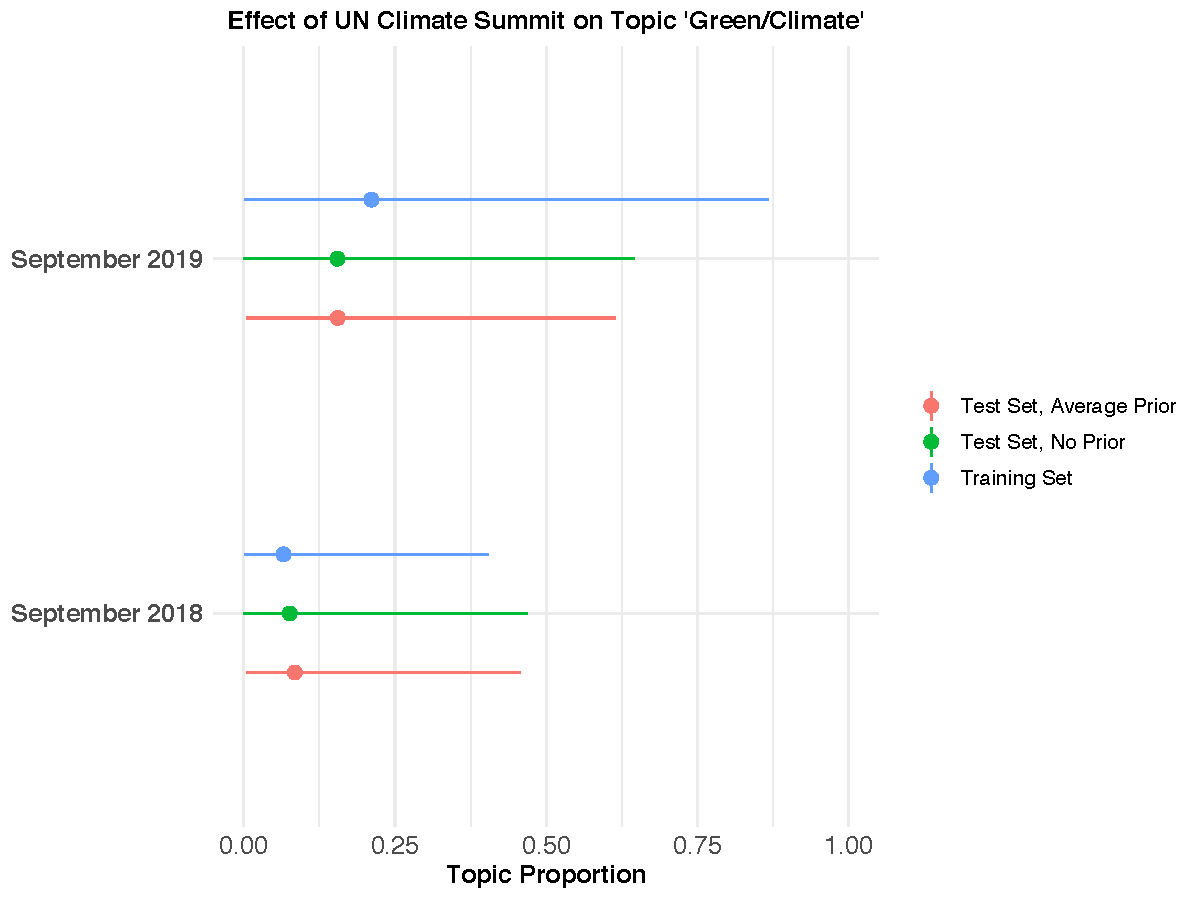
\includegraphics[width=\linewidth]{../plots/presentation/climate_summit_props.pdf}
  \end{subfigure}
  \begin{subfigure}[b]{0.49\linewidth}
    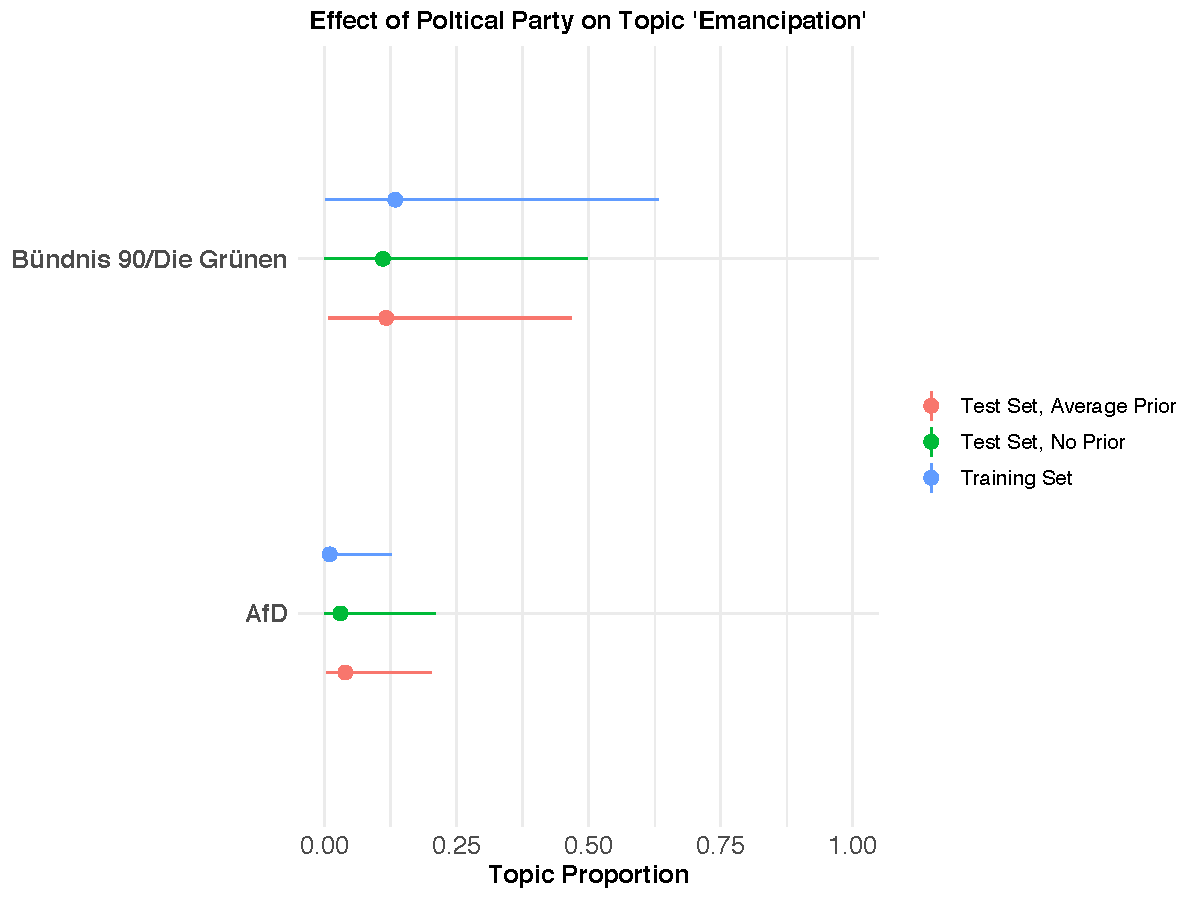
\includegraphics[width=\linewidth]{../plots/presentation/emancipation_props.pdf}
  \end{subfigure}
\end{figure}
\end{frame}

\begin{frame}
\frametitle{Causal Inference}
\framesubtitle{Results (II)}
\begin{itemize}
\item UN Climate Action Summit 2019 held on September 23, 2019
\item As observed, topic associated with climate issues much more prevalent during that time than the year before
\item MAP estimates for different prior specifications on test set rather similar, yet estimated effect for training data much larger
\item Similar results for effect of political party on topic labeled as 'Emancipation': average difference of estimated topic proportions between both parties larger for the training data
\item Additionally: credible intervals on the training data different from those on the test data in both cases
\end{itemize}
\end{frame}

\begin{frame}
\frametitle{Causal Inference}
\framesubtitle{Results (III)}
\begin{itemize}
\item Estimation of treatment effect: determining the average difference of predicted topic proportions between both groups
\begin{figure}[h!]
  \centering
  \captionsetup{justification=centering,margin=2cm}
  \begin{subfigure}[b]{0.4\linewidth}
    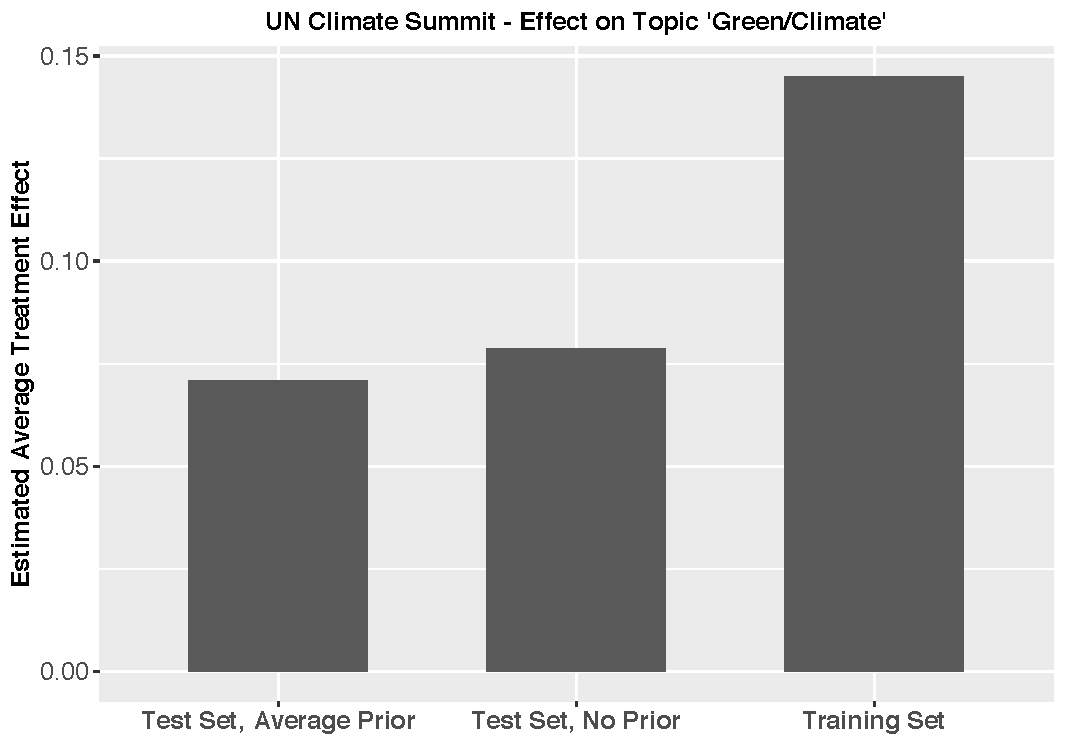
\includegraphics[width=\linewidth]{../plots/presentation/climate_summit_ate.pdf}
  \end{subfigure}
  \begin{subfigure}[b]{0.4\linewidth}
    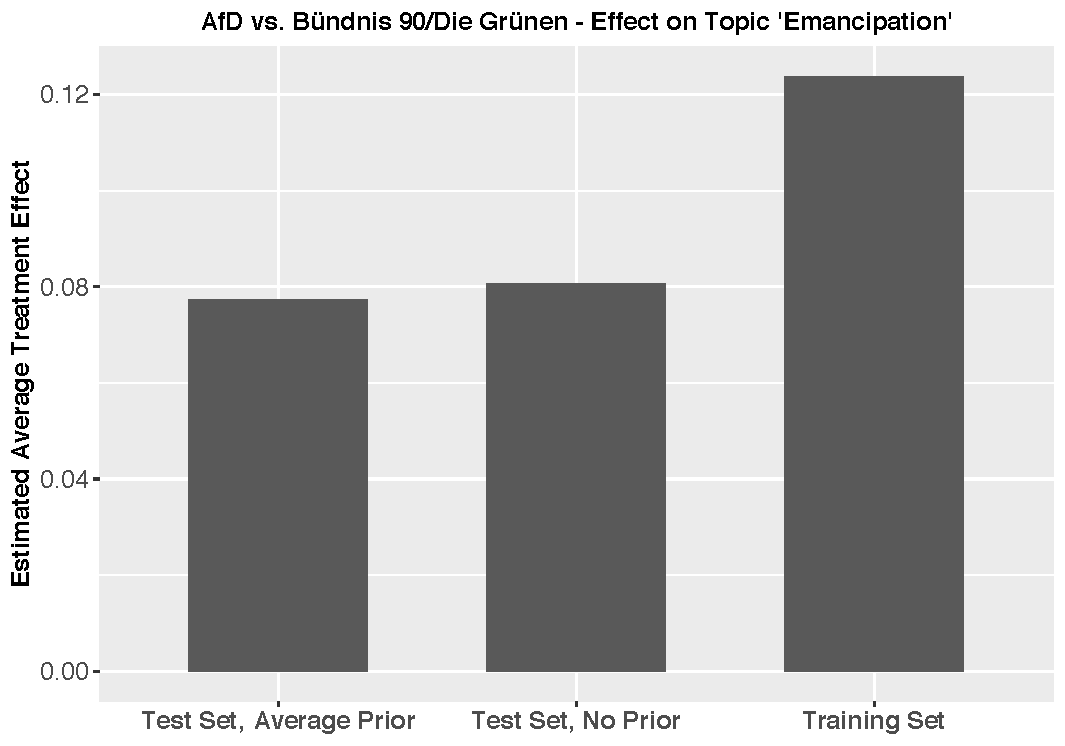
\includegraphics[width=\linewidth]{../plots/presentation/emancipation_ate.pdf}
  \end{subfigure}
\end{figure}
\item Treatment effect larger if "na{\"i}vely" estimated solely on training data in both cases!
\end{itemize}
\end{frame}

\section{Discussion}
\begin{frame}
\frametitle{Discussion}
\framesubtitle{Summary}
\begin{itemize}
\item Creation of broad dataset including large-scale unstructured text and variety of metadata $Rightarrow$ use in future (politological) analyses
\item Exemplification of topic analysis for German parliamentarians' Twitter communication
\item Critical discussion of existing tools and development of new approaches regarding estimation of topic-metadata relationships
\item Detailed illustration of train-test framework for causal inference within the STM
\end{itemize}
\end{frame}

\begin{frame}
\frametitle{Discussion}
\framesubtitle{Suggestions for Future Research}
\begin{itemize}
\item Holistic framework for estimation of topic-metadata relationships $rightarrow$ investigation of effect size and especially importance, for instance through fully Bayesian approach using MCMC
\item Identification of natural experiments for causal inference
\item Research into alternative model designs, beyond STM (and LDA)
\end{itemize}
\end{frame}

\begin{frame}
\frametitle{Bibliography}
\printbibliography
\end{frame}
\end{document}